\documentclass[a4paper, twocolumn, 10pt]{IEEEtran}

\usepackage[utf8]{inputenc}
\usepackage[T1]{fontenc}
\usepackage{float}
\usepackage{hyperref}
\usepackage{graphicx}
\usepackage{booktabs}

\title{Servicios sí, topología no: qué replica un agente LLM del dataset Cloudscape y por qué el prompt engineering no cierra la brecha}
\author{Steven Martinez, Melissa Cobos}
\begin{document}
\maketitle

\begin{abstract}
Construir a mano un catálogo de arquitecturas en la nube a partir de vídeos toma
meses de trabajo especializado: Cloudscape, el mayor inventario público de diseños
sobre AWS, costó más de 18 persona-meses y no se actualiza desde 2023. Este
artículo mide hasta qué punto un agente multimodal de dos etapas puede hacer esa
tarea. Sobre 321 arquitecturas ya catalogadas, el agente reproduce el inventario de
servicios con un F1 de 86,78\,\% y las conexiones con 59,65\,\%. La brecha no
depende del modelo: con la misma entrada, Gemini 3.6 Flash, Gemini 3.1 Pro y Claude
Opus 5.5 quedan entre 59,80 y 61,27 de F1 de conexiones. Tampoco se cierra
reescribiendo las instrucciones ni leyendo mejor la pizarra: doce variantes de
\emph{prompt} no la mueven, y una persona transcribiendo el diagrama aporta 2,27
puntos. Cuando la segunda etapa recibe la referencia como entrada y se le pide
conservar sus conexiones, la reproduce completa: la brecha está en lo que la
pizarra no contiene, y hasta 19 de sus 43 puntos son convenciones de anotación,
sobre todo el sentido de las respuestas. Al sustituir el catálogo curado a mano en
un estudio publicado, su clasificación coincide en el 94,8\,\% de los casos, pero
las cifras que dependen de flujos caen un 28\,\%. Procesar un vídeo cuesta unos
3 céntimos de dólar.
\end{abstract}

\section*{Palabras clave}
Arquitecturas de software, modelos multimodales, cloud, varianza de prompts.


\section{Introducción}

Las decisiones de diseño de los sistemas cloud que están en producción casi nunca
se publican. Un lugar donde sí aparecen es la serie de vídeos \emph{This is My
Architecture} de AWS, en la que un ingeniero dibuja en una pizarra el sistema que
su empresa tiene funcionando y lo explica en pocos minutos. Cloudscape convirtió
396 de esos vídeos en grafos formales y los usó para responder con datos
preguntas que antes se contestaban por intuición: qué servicios se usan de
verdad, con qué se conectan, cuánta variedad hay~\cite{satija2025cloudscape}. El
dataset ya sirve de base a otros trabajos~\cite{santillan2025hpc}.

Construirlo costó más de 18 persona-meses de trabajo iterativo entre seis
anotadores. Ese costo tiene una consecuencia concreta: el dataset se cerró en 2023
y no se ha vuelto a actualizar, aunque la serie siguió publicando vídeos. Cualquier
conclusión que hoy se extraiga de él describe el estado de la práctica de hace
varios años, y el trabajo derivado hereda la misma fecha de corte.

La pregunta natural es si un agente multimodal puede hacer ese trabajo. La
respuesta que encontramos no es un sí ni un no: \textbf{el agente reproduce el
inventario de servicios y no reproduce las conexiones entre ellos}. Reportamos las
dos magnitudes por separado porque el catálogo responde dos clases de preguntas:
las de inventario (qué servicios se usan y con qué frecuencia) dependen del
conjunto de servicios, y las de flujo (cómo se mueven los datos, cuántos pasos
tiene un proceso) dependen de las conexiones. Una cifra media escondería que las
primeras ya se pueden automatizar y las segundas no.

El trabajo aporta cinco resultados:

\begin{enumerate}\itemsep3pt
\item \textbf{La asimetría entre servicios y conexiones}: 27 puntos de F1 sobre
321 arquitecturas, que se repiten con tres modelos de dos proveedores.
\item \textbf{Reescribir el \emph{prompt} no cierra la brecha}: once variantes
caben en 3,61 puntos, del tamaño de lo que el sistema varía por sí solo, y cinco
intervenciones diseñadas a partir del análisis de error tampoco la mueven.
\item \textbf{Dónde está la brecha}: con la referencia como entrada, la segunda
etapa la reproduce completa si se le pide conservar las conexiones recibidas; una
lectura humana de la pizarra solo aporta 2,27 puntos. Lo que falta no está en la
pizarra, y hasta 19 de los 43 puntos son convenciones de anotación.
\item \textbf{Qué le pasa a un estudio publicado} si sus datos se reemplazan por
los del agente: su clasificación se mantiene en el 94,8\,\% de los casos y las
cifras que dependen de flujos caen un 28\,\%.
\item \textbf{Cuánto cuesta}: unos 3 céntimos de dólar por vídeo con el modelo de
producción, unos 13 dólares para todo el dataset.
\end{enumerate}

Para un sistema automatizado, extraer estos grafos va más allá de reconocer logos
en un fotograma. Primero, la oclusión: el presentador tapa el diagrama mientras
habla y la pizarra queda despejada solo por breves instantes. Segundo, la
desconexión multimodal: muchas conexiones se mencionan en voz pero nunca se
dibujan, y contenedores genéricos rotulados como «AWS» esconden varios servicios
nombrados en el audio. Tercero, anotar no es transcribir: el sistema no debe copiar
la pizarra, sino aplicar las reglas de codificación del dataset para decidir cuándo
apegarse a la línea dibujada y cuándo usar el contexto hablado.

\section{Metodología}

El sistema toma la URL de un vídeo y devuelve un archivo .graphml con el esquema de
Cloudscape. Descarga el vídeo con yt-dlp, transcribe el audio con Whisper sobre GPU,
extrae un fotograma cada 10 segundos, elige el mejor fotograma de pizarra y lo envía
junto con la transcripción completa a un agente de dos etapas. Todo lo anterior al
agente es local y no consume cuota de API.

\subsection{Elección del fotograma}

El fotograma elegido es el que reúne a la vez la mayor cantidad de servicios
dibujados, la mayor cantidad de líneas entre ellos y la menor oclusión. Los
servicios se detectan como regiones cuadradas de color vivo cuyo brillo contrasta
con el de un marco de veinte píxeles a su alrededor; las líneas, con un detector de
bordes sobre la misma zona, tapando antes los iconos y con un tope para que el
ruido visual no gane; la oclusión, como la proporción de tonos de piel, que se resta
y es el término con más peso. Las tres medidas se hacen sobre la franja central de
la imagen, donde está la pizarra, pero el fotograma se envía completo. Se descarta
el primer 20\,\% del vídeo y las pantallas de créditos.

\subsection{Dos etapas}

La etapa 1 tiene como objetivo producir un inventario literal de la pizarra: las
entidades dibujadas y las flechas entre ellas, cada una con su etiqueta. La etapa 2
lleva ese inventario al esquema de Cloudscape: normaliza cada servicio al catálogo
del dataset, fusiona los iconos repetidos de un mismo servicio cuando cumplen el
mismo papel y los separa cuando hacen pasos distintos, expande los contenedores
genéricos en los servicios que nombra el audio y ordena las conexiones en flujos con
número de secuencia. Las dos etapas reciben, además de la imagen, la transcripción
del audio, porque parte de la arquitectura solo se describe verbalmente.

Separar las etapas tiene una consecuencia que el diseño buscaba: la entrada de la
etapa 2 se puede sustituir por una lectura humana de la pizarra o por la propia
referencia, y eso permite medir por separado la lectura y la interpretación
(Sección~\ref{sec:oraculo}). La salida de cada etapa se fuerza con un esquema
estructurado, y las llamadas a Gemini usan temperatura 0.

\paragraph{Modelos} El sistema de producción usa \texttt{gemini-3.6-flash} en las
dos etapas. Para comprobar si las conclusiones dependen del modelo repetimos parte
de los experimentos con \texttt{gemini-3.1-pro-preview} y con
\texttt{claude-opus-5-5}. Claude se invoca desde su cliente de línea de comandos,
que no permite fijar la temperatura.

\subsection{Conjunto de evaluación}

Cloudscape tiene 396 arquitecturas. El sistema procesó 370; descartando las que los
autores del dataset marcan como no utilizables y las que no tienen conexiones en la
referencia quedan 321, sobre las que se reportan los resultados globales.

Los experimentos que repiten mediciones (variantes de \emph{prompt}, oráculos y
comparación de modelos) se hacen sobre un subconjunto fijo de \textbf{30
arquitecturas}, el panel. Procesarlo una vez son 30 llamadas, y el nivel gratuito de
la API admitía 20 llamadas por proyecto y día: el tamaño del panel lo fija esa
cuota.

\subsection{Protocolo de evaluación}

El \textbf{protocolo estricto} mide el F1 de servicios sobre el conjunto de tipos de
servicio presentes, con coincidencia exacta y sin contar repeticiones, y el F1 de
aristas sobre el multiconjunto de pares dirigidos (origen, destino), contando cada
línea cuando hay flujos paralelos. Se mide también la exactitud de tipo: entre las
conexiones correctas, qué fracción lleva el tipo de Cloudscape (\texttt{data} o
\texttt{meta}).

El \textbf{protocolo permisivo} mide la calidad del grafo base, sin las convenciones
de anotación. Perdona tres cosas: (i) los subtipos de actor (todo \texttt{User*}
cuenta como \texttt{User}); (ii) las repeticiones de un mismo par; (iii) la
dirección. Si la referencia tiene \texttt{UserConsumerWebMobile}$\rightarrow$%
\texttt{CloudFront}, \texttt{Lambda}$\rightarrow$\texttt{S3},
\texttt{S3}$\rightarrow$\texttt{Lambda} y \texttt{ApiGateway}$\rightarrow$%
\texttt{Lambda}, y el sistema pone otro subtipo de usuario, omite la respuesta de
\texttt{S3} e invierte la de \texttt{ApiGateway}, el estricto da 1 de 4; la regla
(i) lo lleva a 2 de 4, la (ii) reduce la referencia a 3 conexiones y la (iii) acepta
la flecha invertida: 3 de 3. Los dos protocolos puntúan los mismos grafos.

La regla (iii) tiene un límite: un sistema que invirtiera todas las flechas sacaría
un F1 de aristas perfecto. Por eso el permisivo se reporta como cota superior de la
calidad del grafo base, junto al estricto y nunca en su lugar.

\subsection{Piso de ruido}
\label{sec:piso}

Un modelo de lenguaje no devuelve siempre lo mismo ante la misma entrada, ni
siquiera a temperatura 0: de 170 salidas repetidas, ninguna fue idéntica carácter
por carácter. Medimos esa variación con réplicas del panel sin cambiar nada. La
diferencia más pequeña que el diseño distingue del ruido (MDE, con
$\alpha=0{,}05$ y potencia 0,80) es de 3,29 puntos en el F1 de aristas y de 1,76 en
el de servicios. Toda comparación del panel se lee contra ese umbral.

El código, los grafos generados y los \emph{prompts} están en
\url{https://github.com/stevenijm777/aws-architecture-extraction}.

\section{Resultados}

\subsection{Servicios frente a conexiones}
\label{sec:rq1}

\begin{table}[H]
\centering\small
\caption{Desempeño sobre las 321 arquitecturas (protocolo estricto).}
\label{tab:rq1}
\begin{tabular}{lrr}
\toprule
 & Sistema & Referencia\\
\midrule
F1 de servicios        & 86,78 & ---\\
F1 de aristas          & 59,65 & ---\\
Brecha                 & \textbf{27,13} & ---\\
\midrule
Nodos por arquitectura   & 9,15 & 9,11\\
Aristas por arquitectura & 9,04 & 12,42\\
\bottomrule
\end{tabular}
\end{table}

La Tabla~\ref{tab:rq1} contiene el resultado central: 27 puntos separan
identificar los servicios de reconstruir las conexiones, y 307 de las 321
arquitecturas quedan por debajo de la diagonal (Figura~\ref{fig:asimetria}). Los
conteos muestran que el déficit no es una pérdida difusa: los nodos calzan (9,15
contra 9,11, una diferencia de $0{,}12\times$ el MDE) y las aristas quedan por
debajo en 3,38 por arquitectura ($4{,}7\times$ el MDE).

\begin{figure}[H]
\centering
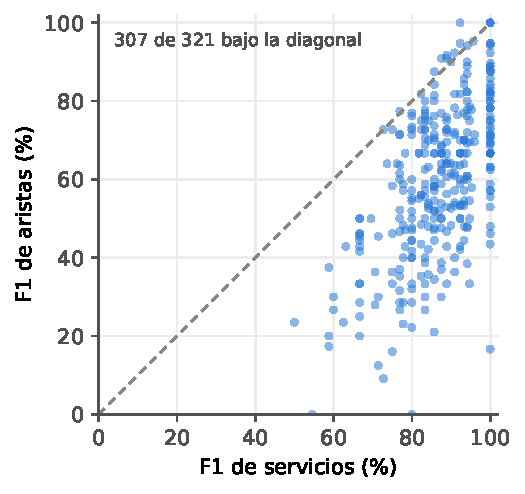
\includegraphics[width=0.78\columnwidth]{imgs/fig_asimetria_standard.pdf}
\caption{F1 de servicios frente a F1 de aristas por arquitectura ($n=321$).}
\label{fig:asimetria}
\end{figure}

La exactitud de tipo es de 61,5\,\%, muy por debajo de lo que daría etiquetar
todo como \texttt{data}, el tipo del 81\,\% de las aristas de la referencia.
La causa es de vocabulario: el \emph{prompt} usa un tercer tipo,
\texttt{control}, que Cloudscape no tiene, y el 30\,\% de las aristas generadas lo
llevan.

\subsection{El \emph{prompt} no cierra la brecha}
\label{sec:rq2}

\begin{table}[H]
\centering\small
\caption{Once variantes de \emph{prompt} de la etapa 2, panel de 30.}
\label{tab:variantes}
\begin{tabular}{lrr}
\toprule
Variante & F1 servicios & F1 aristas\\
\midrule
V7 retorno sobre V6 (c10)          & 88,07 & \textbf{60,10}\\
V6 optimizado (c8)                 & 86,75 & 59,14\\
V6 corregido (c9) --- producción   & 88,06 & 58,99\\
V7 flujos de retorno (c7)          & 86,91 & 58,65\\
V5 ruteo estricto (c8)             & 86,78 & 58,45\\
V8 actores y retornos              & 86,21 & 58,40\\
V6 corregido (c10)                 & 88,47 & 58,10\\
V5 ruteo estricto (c7)             & 86,65 & 58,08\\
V6 corregido (c7)                  & 85,92 & 57,52\\
V4 anti-alucinación (c8)           & 85,62 & 57,10\\
V4 \emph{few-shot} dinámico        & 88,03 & 56,49\\
\midrule
\textbf{Rango}                     & \textbf{2,84} & \textbf{3,61}\\
MDE ($n=30$)                       & 1,76 & 3,29\\
\bottomrule
\end{tabular}
\end{table}

Entre la mejor y la peor de las once variantes de la Tabla~\ref{tab:variantes} hay
3,61 puntos de F1 de aristas, apenas por encima de los 3,29 que el sistema se mueve
solo. Comparar el extremo mejor contra el peor da 10 victorias, 7 derrotas y 13
empates ($p=0{,}629$).

Siguiendo a Arcuri y Briand~\cite{Arcuri2011StatisticalSE}, reportamos el tamaño de
efecto con su intervalo y no solo el valor $p$. Sobre las 55 comparaciones entre
variantes, el $\hat{A}_{12}$ de Vargha y Delaney va de 0,452 a 0,553, y los 55
intervalos de confianza por \emph{bootstrap} contienen el 0,5, con un ancho medio de
0,110. En la misma prueba y sobre el mismo panel, el brazo de oráculo de la
Sección~\ref{sec:oraculo} da $\hat{A}_{12}=0{,}861$ $[0{,}794;\,0{,}927]$: el diseño
detecta diferencias cuando las hay. Lo que sostenemos es que ninguna diferencia
entre variantes es detectable, no que sean equivalentes. Ninguna comparación
sobrevive tampoco a la corrección de Bonferroni o de Holm (el $p$ mínimo es 0,0074
frente a un $\alpha$ corregido de 0,00091), una corrección que esos autores no
recomiendan y que reportamos solo como control.

\begin{table}[H]
\centering\small\setlength{\tabcolsep}{4pt}
\caption{Intervenciones dirigidas, panel de 30. Diferencia pareada con su línea
base de producción.}
\label{tab:intervenciones}
\begin{tabular}{lrrr}
\toprule
Intervención & $\Delta$ aristas & $\times$MDE & signos\\
\midrule
Evidencia visual (Hough)          & $-1{,}60$ & $0{,}49$ & $p=0{,}55$\\
V8 · actores y retornos           & $-0{,}59$ & $0{,}18$ & $p=0{,}61$\\
Auditoría de retornos             & $+1{,}20$ & $0{,}36$ & $p=1{,}00$\\
\emph{Few-shot} RAG               & $-2{,}50$ & $0{,}76$ & $p\approx0{,}33$\\
V9 · conexiones autoritativas     & $+0{,}43$ & $0{,}13$ & $p=1{,}00$\\
\bottomrule
\end{tabular}
\end{table}

Las cinco intervenciones de la Tabla~\ref{tab:intervenciones} se diseñaron a partir
de los errores más frecuentes, y ninguna alcanza el umbral. En dos de
ellas se verificó que el mecanismo funcionaba: la auditoría de retornos generó
propuestas válidas en el 100\,\% de los casos y V8 sí recuperó nodos actor. La
quinta, V9, es la que corrige el experimento de oráculo (Sección~\ref{sec:oraculo});
en producción da $+0{,}43$ puntos y $+0{,}03$ en una segunda corrida.

\subsection{Dónde está la brecha}
\label{sec:oraculo}

El experimento cambia una sola cosa: de dónde sale la descripción de la pizarra que
recibe la etapa 2. En \textbf{producción} la genera la etapa 1; en el \textbf{brazo
A} la escribió una persona mirando solo la pizarra, sin audio y sin ver la
referencia; en el \textbf{brazo B} es la referencia de Cloudscape. El \emph{prompt},
la imagen, el audio y el evaluador no cambian.

\begin{table}[H]
\centering\small\setlength{\tabcolsep}{4pt}
\caption{Experimento de oráculo con Flash, panel de 30. Media de las réplicas
disponibles.}
\label{tab:oraculos}
\begin{tabular}{lrrr}
\toprule
Entrada de la etapa 2 & \emph{Prompt} & F1 svc & F1 aristas\\
\midrule
Etapa 1 (producción, 4 réplicas) & V6 & 87,10 & 58,13\\
A · transcripción humana         & V6 & 87,82 & 60,40\\
B · \emph{ground truth}          & V6 & 99,57 & 82,17\\
B · \emph{ground truth}          & V9 & 99,72 & 99,54\\
\bottomrule
\end{tabular}
\end{table}

\paragraph{Leer mejor la pizarra no ayuda.} El brazo A no se despega de producción:
$+2{,}27$ puntos, 17 victorias, 7 derrotas, $p=0{,}064$, dentro del MDE
(Tabla~\ref{tab:oraculos}). La transcripción humana, puntuada directamente contra la
referencia, da 57,60 de F1 de conexiones, igual que el sistema completo: una persona
sin oclusión y sin límite de tiempo también dibuja 8,63 conexiones donde la
referencia tiene 12,03. Esas conexiones no están dibujadas.

\paragraph{Con la respuesta delante, el \emph{prompt} era el cuello.} En el brazo B
la etapa 2 recibe la referencia y aun así se queda en 82,17. Comparando entrada y
salida arista por arista, Flash conserva los nodos (263 donde hay 262) y pierde 86
aristas: en 59 la entrada trae una conexión en los dos sentidos y la salida solo
uno, y en 22 la entrada repite un mismo par y la salida lo emite una vez. El
\emph{prompt} de producción pide justificar cada arista con una flecha dibujada o
una frase del audio y tratar los flujos como unidireccionales salvo evidencia
contraria; las conexiones del oráculo no traen descripción, y el modelo conserva el
sentido que el audio narra y descarta el otro. La variante V9 declara autoritativas
las conexiones recibidas: una arista por conexión, sin descartar sentidos ni
repeticiones. Con ella Flash reproduce la referencia completa en una corrida y
pierde 0,92 puntos en la segunda. Quitar solo la regla de unidireccionalidad, sin
el resto de V9, no tiene efecto (81,86).

\begin{figure}[H]
\centering
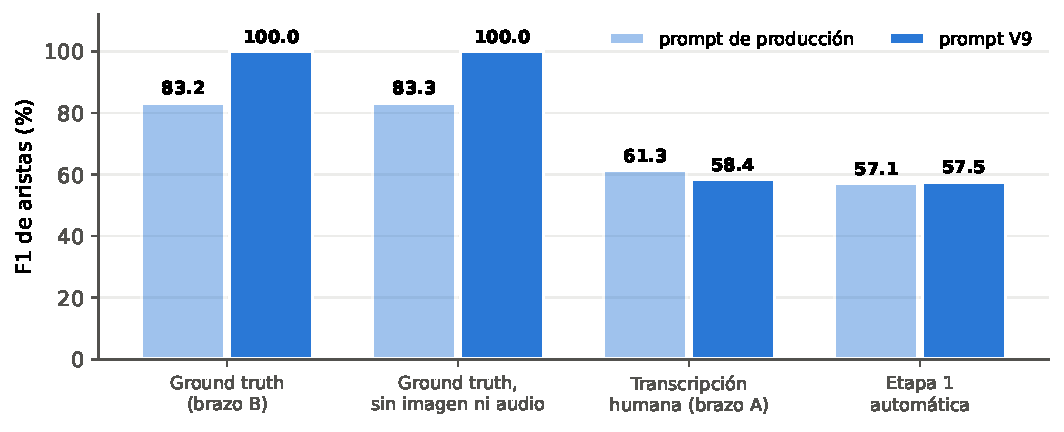
\includegraphics[width=\columnwidth]{imgs/fig_v9_cuatro_condiciones.pdf}
\caption{F1 de aristas de Flash con el \emph{prompt} de producción y con V9. El
cambio solo altera el resultado cuando la entrada trae las conexiones.}
\label{fig:v9}
\end{figure}

\paragraph{Fuera del oráculo, V9 no cambia nada.} En producción da 57,55 y 57,15
frente a 57,12, y con los demás modelos queda en el mismo rango (Pro 57,52, Claude
56,18, Gemini 4 Argon 59,19); en el brazo A, 58,45 frente a 61,27 y 60,40, porque copiar la
lectura humana le quita a la etapa 2 la libertad de completarla con el audio
(Figura~\ref{fig:v9}). La etapa 2 transporta todas las conexiones que recibe:
reescribir sus instrucciones no cierra la brecha porque las conexiones que faltan
no llegan en su entrada. El audio aporta, pero poco: quitárselo a la etapa 2 en el
brazo A baja el F1 de aristas de 60,40 a 56,72.

\paragraph{Cuánto de la brecha es convención.} Cloudscape documenta dos reglas de
anotación que la pizarra no muestra: cuando la descripción verbal no coincide con
el dibujo, la referencia sigue a la verbal, y los flujos registran el grafo completo
de peticiones \emph{y respuestas}~\cite{satija2025cloudscape}. Las reglas (ii) y
(iii) del protocolo permisivo perdonan justamente las repeticiones y el sentido de
vuelta. En producción, el permisivo lleva el F1 de aristas de 57,12 a 76,64, y la
lectura humana de 57,60 a 75,81: de los 43 puntos que separan al sistema del techo,
hasta 19 son convención y unos 23 son pares de servicios que no aparecen en la
pizarra. Es una cota superior, por el límite de la regla (iii).

\subsection{¿Depende del modelo?}
\label{sec:modelos}

\begin{table}[H]
\centering\footnotesize\setlength{\tabcolsep}{3pt}
\caption{F1 de aristas con tres modelos, panel de 30. «Etapa 1» puntúa la lectura
de la pizarra (solo la imagen) contra la referencia; las demás columnas, la salida
de la etapa 2. Media de las réplicas disponibles.}
\label{tab:modelos}
\begin{tabular}{lrrrr}
\toprule
 & Etapa 1 & Brazo A & Brazo B (V6) & Brazo B (V9)\\
\midrule
Persona                & 57,60 & ---   & ---   & ---\\
Gemini 3.6 Flash       & 53,34 & 60,84 & 82,17 & 99,54\\
Gemini 3.1 Pro         & 52,72 & 59,80 & 69,81 & 94,12\\
Claude Opus 5.5        & 52,31 & 60,75 & 82,89 & 97,62\\
\bottomrule
\end{tabular}
\end{table}

Un modelo más fuerte no reduce la brecha en ninguna etapa (Tabla~\ref{tab:modelos}).
En la etapa 1, las lecturas de los tres modelos quedan entre 52,31 y 53,34 contra la
referencia, y la humana las supera por entre 4,3 y 5,3 puntos. En la etapa 2, con la
misma transcripción manual, Pro queda $-1{,}47$ puntos por debajo de Flash
(IC$_{95\%}$ $[-5{,}63;\,+2{,}60]$) y Claude $-0{,}52$ (IC$_{95\%}$
$[-4{,}90;\,+3{,}75]$); Gemini 4 Argon, probado con la misma entrada, queda en 60,40.
Lo que cambia es el conteo: Pro y Claude dibujan 11,40 y
11,20 aristas por arquitectura, cerca de las 12,03 de la referencia, frente a 9,00
de Flash; ganan recall, pierden precisión y el F1 no se mueve. El subdibujado de la
Tabla~\ref{tab:rq1} es del modelo de producción; lo que comparten los tres es no
acertar cuáles conexiones faltan.

Pro muestra además el caso contrario a V9. En el brazo B con el \emph{prompt} de
producción añade 113 aristas que no están en la referencia e inventa 19 servicios, y
65 de esas aristas son las mismas que dibuja en el brazo A, donde solo tiene la
lectura de la pizarra. Sin imagen ni audio sube a 87,59 y 88,75 en dos corridas: con
la respuesta delante, el modelo la reescribe a partir del dibujo y la narración.

El protocolo permisivo no revela diferencias escondidas: sobre la misma entrada, los
tres modelos quedan entre 93,0 y 94,0 en servicios y entre 76,6 y 79,1 en aristas
(Figura~\ref{fig:permisivo}). Con V9, las segundas corridas de los tres modelos
difieren de las primeras en menos de un punto.

\begin{figure}[H]
\centering
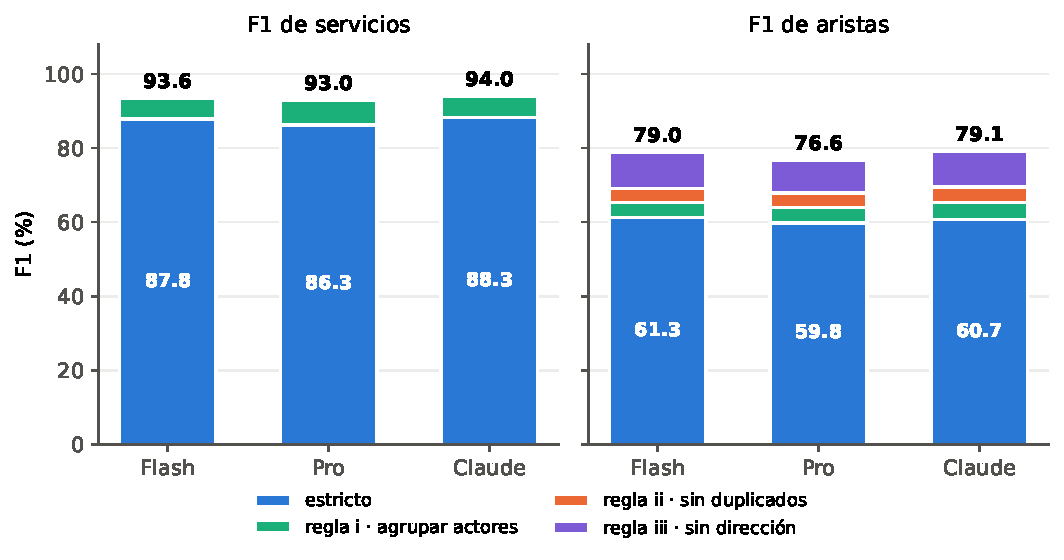
\includegraphics[width=\columnwidth]{imgs/fig_permisivo_por_modelo.pdf}
\caption{Protocolo estricto y aporte de cada regla del permisivo, por modelo, con
la misma transcripción manual como entrada (brazo A).}
\label{fig:permisivo}
\end{figure}

\subsection{Costo}
\label{sec:costo}

\begin{table}[H]
\centering\footnotesize\setlength{\tabcolsep}{3pt}
\caption{Costo por vídeo a las tarifas publicadas en octubre de 2026. Tokens medios
de la etapa 2; el costo suma las dos etapas cuando ambas se midieron.}
\label{tab:costo}
\begin{tabular}{lrrrr}
\toprule
Modelo & Entrada & Salida & USD/vídeo & 396 vídeos\\
\midrule
Gemini 3.6 Flash   & 4\,802  & 3\,845 & 0,033 & 13\\
Gemini 3.1 Pro     & 4\,802  & 5\,851 & 0,145 & 58\\
Claude Opus 5.5    & 10\,371 & 3\,875 & 0,139$^{*}$ & ---\\
Gemini 4 Argon     & 5\,400  & 2\,019 & 0,031$^{*}$ & ---\\
\bottomrule
\end{tabular}
\\[2pt]\raggedright\scriptsize $^{*}$Solo la etapa 2. Claude: costo equivalente de API
informado por su cliente. Argon: tarifa vigente hasta noviembre de 2026.
\end{table}

Con el modelo de producción, procesar un vídeo cuesta unos 3 céntimos de dólar
(Tabla~\ref{tab:costo}) y rehacer las 396 arquitecturas, unos 13 dólares, frente a
los 18 persona-meses del catálogo original. La salida incluye los tokens de
razonamiento, que son el 52\,\% del costo de la etapa 2 con Flash y el 63\,\% con
Pro; la etapa 1 de Pro se midió sobre 7 vídeos. La tarifa de Flash es promocional
hasta finales de 2026 y se duplica después; aun así, mantener el catálogo al día con
los vídeos nuevos de la serie, unos 20 al mes en su punto más alto, cuesta menos de
un dólar al mes.

\subsection{¿Sirven estos grafos en un estudio publicado?}
\label{sec:downstream}

Ejecutamos el código de Santillán y Abad~\cite{santillan2025hpc}, que clasifica cada
arquitectura como HPC, Edge, ambas o ninguna a partir de los servicios presentes,
sustituyendo su corpus anotado a mano por los grafos del sistema sobre las mismas
385 arquitecturas. Lo único que cambia es quién leyó la pizarra.

\begin{table}[H]
\centering\small
\caption{Clasificación HPC/Edge con los grafos del sistema (385 arquitecturas).}
\label{tab:downstream}
\begin{tabular}{lr}
\toprule
Resultado & Valor\\
\midrule
Coincidencia de clasificación     & 365/385 = 94,8\,\%\\
Top-10 preservado (HPC / Edge / None) & 7 / 8 / 9\\
\bottomrule
\end{tabular}
\end{table}

En ese clasificador basta que falte un servicio para que una arquitectura cambie de
categoría, y aun así coincide en el 94,8\,\% de los casos. La mayoría de los
desacuerdos se explica por un único nodo de actor perdido (un dispositivo, no un
servicio de AWS). En la parte del estudio que depende de la topología, el conteo de
\emph{workflows}, la conclusión cualitativa de los autores se mantiene, pero las
medias caen alrededor de un 28\,\%, porque el sistema subcuenta \emph{workflows}
igual que subdibuja aristas.

El sistema procesa además 61 arquitecturas que Cloudscape no cubre, 33 de ellas de
2024. Clasificadas con la misma regla, la proporción de arquitecturas Edge pasa de
25,5\,\% a 27,4\,\% entre las 457 resultantes. Es una actualización del catálogo, no
una tendencia: los autores advierten que la variación anual de la serie puede
deberse a la curaduría del canal.

\section{Trabajo relacionado}

La reconstrucción de arquitecturas recupera el diseño de un sistema a partir de su
código fuente~\cite{Ducasse2009SAR}, y las comparaciones de técnicas automáticas
encuentran que incluso la mejor tiene una precisión sorprendentemente baja al
recuperar la estructura~\cite{Garcia2013ComparativeSAR}. Este trabajo no parte del
código sino de vídeos en los que un ingeniero dibuja y explica su arquitectura.
Los propios autores de Cloudscape probaron modelos generativos multimodales con
ejemplos y ajuste de \emph{prompts} para ayudar a la anotación, con baja
precisión~\cite{satija2025cloudscape}; aquí medimos por separado qué parte de la
tarea ya se puede automatizar y por qué la otra no.

Los modelos de lenguaje razonan peor sobre grafos a medida que estos se vuelven más
complejos, y el beneficio de las técnicas de \emph{prompting} disminuye en los
problemas más difíciles~\cite{Fatemi2024TalkLikeAGraph, Wang2023NLGraph}. Esa
literatura llevaría a esperar que el límite estuviera en el modelo o en la
instrucción; nuestros resultados lo sitúan en la entrada. Para no confundir
sensibilidad al texto con mejora real evaluamos varias instrucciones y no una
sola~\cite{Mizrahi2024MultiPromptEval}, con las pruebas y tamaños de efecto que
recomiendan Arcuri y Briand~\cite{Arcuri2011StatisticalSE}. El experimento de
oráculo sigue la idea de evaluar una etapa suponiendo perfecta la anterior, como en
la evaluación de reparación automática con localización de fallos
perfecta~\cite{Liu2019FaultLocalizationBias}.

\section{Limitaciones}

Todas las cifras se comparan contra una única anotación de referencia, y casi toda
la brecha corresponde a conexiones que no están en la pizarra; no sabemos qué parte
de ellas es recuperable del vídeo y qué parte es criterio del anotador. Los
experimentos con otros modelos se hicieron sobre el panel de 30, varias condiciones
tienen una sola corrida, a Claude no se le puede fijar la temperatura y la
transcripción manual la hizo una sola persona.

\section{Conclusiones}

Un agente multimodal de dos etapas ya reproduce el inventario de servicios de una
arquitectura (86,78 de F1) y no reproduce sus conexiones (59,65). La extracción
automática sirve hoy para las preguntas que dependen del conjunto de servicios, y su
costo, unos 13 dólares por todo el catálogo, permite mantenerlo al día; las
preguntas que dependen de flujos siguen necesitando revisión humana.

La brecha no se cierra cambiando el modelo, reescribiendo las instrucciones ni
leyendo mejor la pizarra. Cuando la segunda etapa recibe las conexiones correctas
las transporta todas; las que faltan no están en lo que el sistema ve, y una parte
importante son convenciones de anotación, como registrar la respuesta de cada
petición. Quedan dos líneas de trabajo: medir el acuerdo entre dos anotadores sobre
un subconjunto del dataset, para saber cuánto del desacuerdo es error del sistema, y
tratar la narración del vídeo como fuente primaria de conexiones y no como contexto
de apoyo.

\bibliographystyle{ieeetr}
\bibliography{referencias}

\end{document}
